\setcounter{section}{21}

\section{Lecture 22: March 17}


\subsection*{Last time}
\begin{itemize}
	\item Collinearity (JF chapter 13, RD 8.3.2)
\item Principal component analysis (JF 13.1.1, RD 8.3.4)
\end{itemize}


\subsection*{Today}
\begin{itemize}
	\item Midterm exam review
	\item Biased estimation (JF 13.2.3, CG's notes)
	\begin{itemize}
		\item Ridge regression
		\item Lasso regression
	\end{itemize}
\end{itemize}

\subsubsection*{Additional reference}
\href{https://math.bu.edu/people/cgineste/classes/ma575/p/w14_1.pdf}{Lecture notes} by Cedric Ginestet

\subsection*{Ridge Regression}

Ridge regression and the Lasso regression are two forms of \underline{regularized regression}.
These methods can be used to alleviate the consequences of multicollinearity.

\begin{enumerate}
	\item When variables are highly correlated, a large coefficient in one variable may be alleviated by a large coefficient in another variable, which is negatively correlated to the former.
	\item Regularization imposes an upper threshold on the values taken by the coefficients, thereby producing a more parsimonious solution, and a set of coefficients with smaller variance.
\end{enumerate}

\subsubsection*{Constrained optimization}

Ridge regression is motivated by a constrained minimization problem, which can be formulated as
$$
\begin{aligned}
&\hat{\beta}^{ridge} = \argmin\limits_{\beta \in \mathbb{R}^p} \sum\limits_{i = 1}^n(y_i - \vecc{x}_i\transpose \beta)^2\\
&\mbox{subject to } ||\beta||_2^2 = \sum\limits_{j = 1}^p \beta_j^2 \le t \\
\end{aligned}
$$
for $t \ge 0$.  

Use a Lagrange multiplier, we can rewrite the formula as
$$
\hat{\beta}^{ridge} =\argmin\limits_{\beta \in \mathbb{R}^p} \{  \sum\limits_{i = 1}^n(y_i - \vecc{x}_i\transpose \beta)^2 + \lambda \sum\limits_{j = 1}^p \beta_j^2\}
$$
for $\lambda \ge 0$ and where there is a one-to-one correspondence between $t$ and $\lambda$.
$\lambda$ is an arbitrary constant usually referred to as the ``ridge constant''.

\subsubsection*{Analytical solutions}
The ridge-regression estimator has analytical solution
$$
\hat{\beta}^{ridge} = (\vecc{X}\transpose\vecc{X} + \lambda \vecc{I})^{-1} \vecc{X}\transpose \vecc{Y}
$$
This is obtained by differentiating the objective function with respect to $\beta$ and set it to $0$:
$$
\begin{aligned}
&\frac{\partial}{\partial \beta} \{(\vecc{Y} - \vecc{X}\beta)\transpose (\vecc{Y} - \vecc{X}\beta) +\lambda \vecc{\beta}\transpose \vecc{\beta}\}\\
=& 2(\vecc{X}\transpose \vecc{X}) \beta - 2 \vecc{X}\transpose \vecc{Y} + 2\lambda \beta \\
=& 0\\
\end{aligned}
$$
Therefore,
$$
(\vecc{X}\transpose\vecc{X} + \lambda \vecc{I})\vecc{\beta} = \vecc{X}\transpose\vecc{Y}
$$

Since we are adding a positive constant to the diagonal of $\vecc{X}\transpose\vecc{X}$, we  are , in general, producing an invertible matrix, $\vecc{X}\transpose\vecc{X} + \lambda\vecc{I}$ even if $\vecc{X}\transpose\vecc{X}$ is singular.  Historically, this particular aspect of ridge regression was the main motivation behind the adoption of this particular extension of OLS theory.

The ridge regression estimator is related to the classical OLS estimator, $\hat{\beta}^{OLS}$, in the following manner
$$
\hat{\beta}^{ridge}  = \left[\vecc{I} + \lambda (\vecc{X}\transpose\vecc{X})^{-1}\right] ^{-1} \hat{\beta}^{OLS},
$$
assuming $\vecc{X}\transpose\vecc{X}$ is non-singular.  This relationship can be verified by applying the definition of $\hat{\beta}^{OLS}$,
$$
\begin{aligned}
\hat{\beta}^{ridge}  &= \left[\vecc{I} + \lambda (\vecc{X}\transpose\vecc{X})^{-1}\right] ^{-1} (\vecc{X}\transpose\vecc{X})^{-1} \vecc{X}\transpose\vecc{Y}\\
&=(\vecc{X}\transpose\vecc{X} + \lambda \vecc{I})^{-1} \vecc{X}\transpose \vecc{Y}\\
\end{aligned}
$$
using the fact $\vecc{B}^{-1}\vecc{A}^{-1} = \vecc{(AB)}^{-1}$.

Moreover, when $\vecc{X}$ is composed of orthonormal variables, such that $\vecc{X}\transpose\vecc{X} = \vecc{I}_p$, it then follows that 
$$
\hat{\beta}^{ridge} = \frac{1}{1 + \lambda} \hat{\beta}^{OLS}
$$

\subsubsection*{Bias and variance of ridge estimator}
Ridge estimation produces a biased estimator of the true parameter $\beta$.
With the definition of $\hat{\beta}^{ridge}$ and the model assumption $\Expected{\vecc{Y}|\vecc{X}} = \vecc{X}\vecc{\beta}$, we obtain,
$$
\begin{aligned}
\Expected{\hat{\beta}^{ridge} | \vecc{X}} &= (\vecc{X}\transpose\vecc{X} + \lambda \vecc{I})^{-1} \vecc{X}\transpose \vecc{X\beta}\\
&= (\vecc{X}\transpose\vecc{X} + \lambda \vecc{I})^{-1}  (\vecc{X}\transpose \vecc{X} + \lambda \vecc{I} - \lambda \vecc{I}) \vecc{\beta}\\
&= \beta - \lambda(\vecc{X}\transpose\vecc{X} + \lambda \vecc{I})^{-1} \vecc{\beta}\\
\end{aligned}
$$
where the bias of the ridge estimator is proportional to $\lambda$. 
The variance of the ridge estimator is
$$
\Var{\hat{\beta}^{ridge} | \vecc{X}} = \sigma^2 (\vecc{X}\transpose\vecc{X} + \lambda \vecc{I})^{-1} (\vecc{X}\transpose\vecc{X})  (\vecc{X}\transpose\vecc{X} + \lambda \vecc{I})^{-1}.
$$
When $\lambda$ increases, the inverted term $(\vecc{X}\transpose\vecc{X} + \lambda \vecc{I})^{-1}$ is increasingly dominated by $\lambda \vecc{I}$.
The variance of the ridge estimator, therefore, is a decreasing function of $\lambda$.
This result is intuitively reasonable because the estimator itself is driven toward $\vecc{0}$.

\subsubsection*{Variance-bias tradeoff}
The mean-squared error of an estimator can be decomposed into the sum of its squared bias and sampling variance.
$$
\begin{aligned}
MSE(\hat{\theta}) &= \Expected{(\hat{\theta} - \theta)^2} = \textbf{E}(\hat{\theta}^2) + \theta^2 - 2 \theta\textbf{E}(\hat{\theta}) \\
Bias^2(\hat{\theta}) &= \left[ \textbf{E}(\hat{\theta}) - \theta\right]^2 = \textbf{E}^2(\hat{\theta}) + \theta^2 - 2 \theta\textbf{E}(\hat{\theta}) \\
\text{Var}(\hat{\theta}) &= \textbf{E}(\hat{\theta}^2) - \textbf{E}^2(\hat{\theta})\\
\end{aligned}
$$
Therefore
$$
MSE(\hat{\theta}) = Bias^2(\hat{\theta}) + \text{Var}(\hat{\theta})
$$
The essential idea here is to trade a small amount of bias in the coefficient estimates for a large reduction in coefficient sampling variance.
Hoerl and Kennard (1970) prove that it is always possible to choose a positive value of the ridge constant $\lambda$ so that the mean-squared error of the ridge estimator is less than the mean-squared error of the least-squares estimator.
These ideas are illustrated heuristically in Figure~\ref{fig:13_9}
%
\begin{figure}[H]
	\begin{center}
		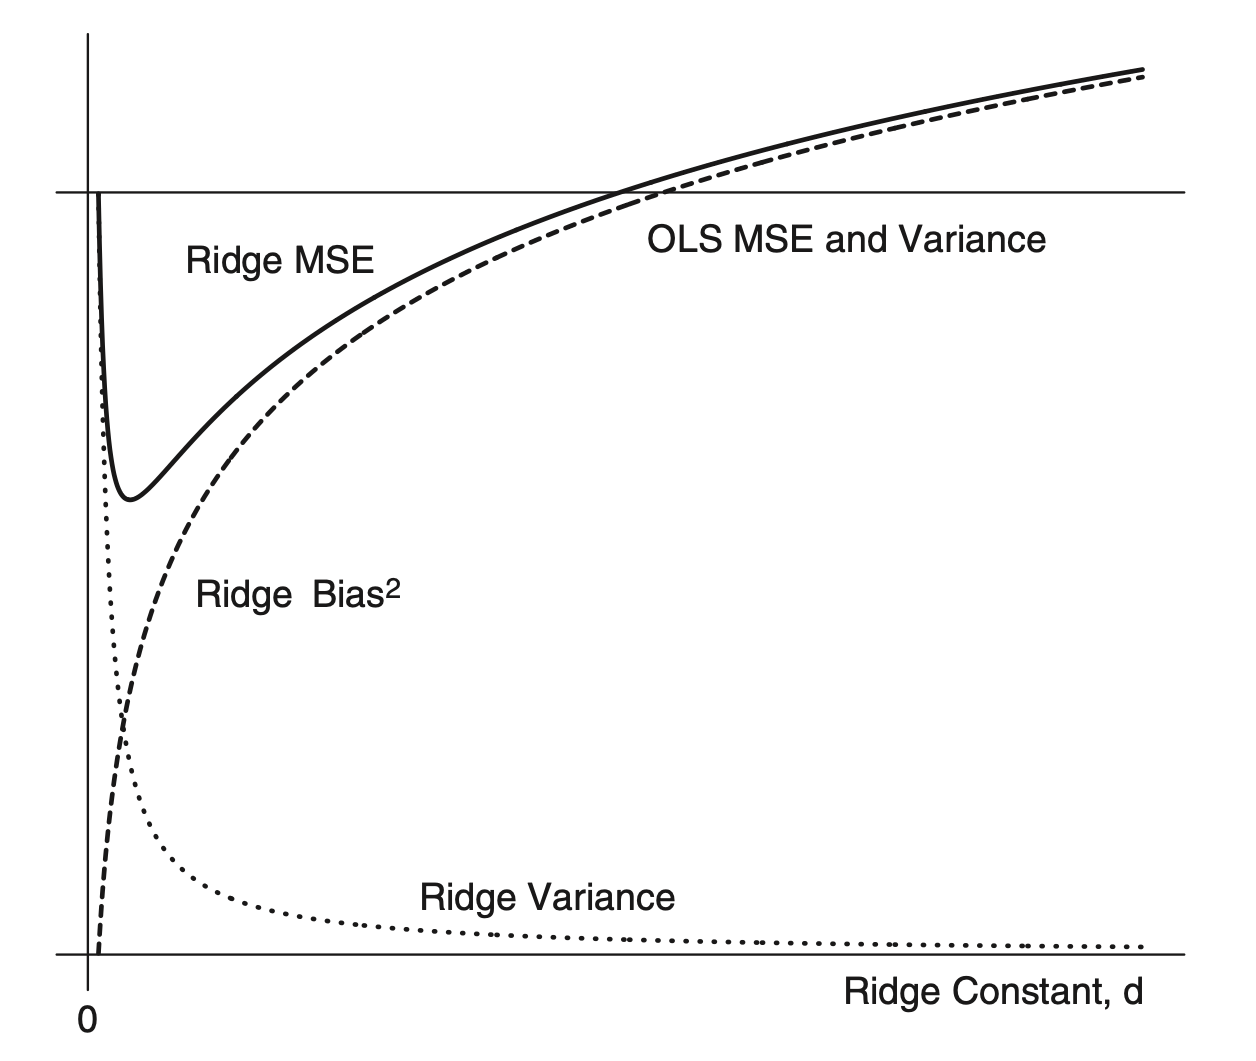
\includegraphics[width=0.7\textwidth]{Lecture22/JF_13_9}
		\caption{
			Trade-off of bias and against variance for the ridge-regression estimator.  
			The horizontal line gives the variance of the least-squares (OLS) estimator; because the OLS estimator is unbiased, its variance and mean-squared error are the same.
			The broken line shows the squared bias of the ridge estimator as an increasing function of the ridge constant $d$ (i.e.~$\lambda$ in our notes).
			The dotted line shows the variance of the ridge estimator.
			The mean-squared error (MSE) of the ridge estimator, given by the heavier solid line, is the sum of its variance and squared bias.
			For some values of $d$, the MSE error of the ridge estimator is below the variance of the OLS estimator.
			JF Figure 13.9.}
		\label{fig:13_9}
	\end{center}
\end{figure}
%

\subsection*{Lasso regression}
We have seen that ridge regression essentially re-scales the OLS estimates.
The lasso, by contrast, tries to produce a {\it sparse} solution, in the sense that several of the slope parameters will be set to zero.

\subsubsection*{Constrained optimization}
Different from the $L_2$ penalty for ridge regression, the Lasso regression employs $L_1$-penalty.
$$
\begin{aligned}
	&\hat{\beta}^{lasso} = \argmin\limits_{\beta \in \mathbb{R}^p} \sum\limits_{i = 1}^n(y_i - \vecc{x}_i\transpose \beta)^2\\
	&\mbox{subject to } ||\beta||_1 = \sum\limits_{j = 1}^p |\beta_j| \le t \\
\end{aligned}
$$
for $t \ge 0$; which can again be re-formulated using the Lagrangian for the $L_1$-penalty,
$$
\hat{\beta}^{lasso} =\argmin\limits_{\beta \in \mathbb{R}^p} \{  \sum\limits_{i = 1}^n(y_i - \vecc{x}_i\transpose \beta)^2 + \lambda \sum\limits_{j = 1}^p |\beta_j|\}
$$
where $\lambda > 0$ and, as before, there exists a one-to-one correspondence between $t$ and $\lambda$.

\subsubsection*{Parameter estimation}
Contrary to ridge regression, the Lasso does not have a closed-form solution.
The $L_1$-penalty makes the solution non-linear in $y_i$'s.
The above constrained minimization is a \underline{quadratic programming} problem, for which many solvers exist.

\subsection*{Choice of Hyperparameters}
\subsubsection*{Regularization parameter}

The choice of $\lambda$ in both ridge and lasso regressions is more of an art than a science.
This parameter can be constructed as a complexity parameter, since as $\lambda$ increases, less and less effective parameters are likely to be included in both ridge and lasso regressions.
Therefore, one can adopt a model selection perspective and compare different choices of $\lambda$ using cross-validation or an information criterion.
That is, the value of $\lambda$ should be chosen adaptively, in order to minimize an estimate of the expected prediction error (as in cross-validation), for instance,
which is well approximated by AIC.
We will discuss model selection in more detail later.

\subsubsection*{Bayesian perspective}
The penalty terms in ridge and lasso regression can also be justified, using a Bayesian framework, whereby these terms arise as aresult of the specification of a particular prior distribution on the vector of slope parameters.

\begin{enumerate}
	\item The use of an $L_2$-penalty in multiple regression is analogous to the choice of a Normal prior on the $\beta_j$'s, in Bayesian statistics.
	$$
	\begin{aligned}
		y_i  &\distas{iid} \mathcal{N}(\beta_0 + \vecc{x}_i\transpose\beta, \sigma^2), \quad  i = 1, \dots, n\\
		\beta_j  &\distas{iid} \mathcal{N}(0, \tau^2), \quad j = 1, \dots, p\\
	\end{aligned}
	$$
	\item Similarly, the use of an $L_1$-penalty in multiple regression is analogous to the choice of a Laplace prior on the $\beta_j$'s, such that
	$$
	\begin{aligned}
	\beta_j  &\distas{iid} Laplace(0, \tau^2), \quad j = 1, \dots, p\\
	\end{aligned}	
	$$
\end{enumerate}
In both cases, the value of the hyperparameter, $\tau^2$, will be inversely proportional to the choice of the particular value for $\lambda$.
For ridge regression, $\lambda$ is exactly equal to the shrinkage parameter of the hierarchical model, $\lambda = {\sigma^2}/{\tau^2}$.









